\chapter{Psalm 9}

\begin{figure}
  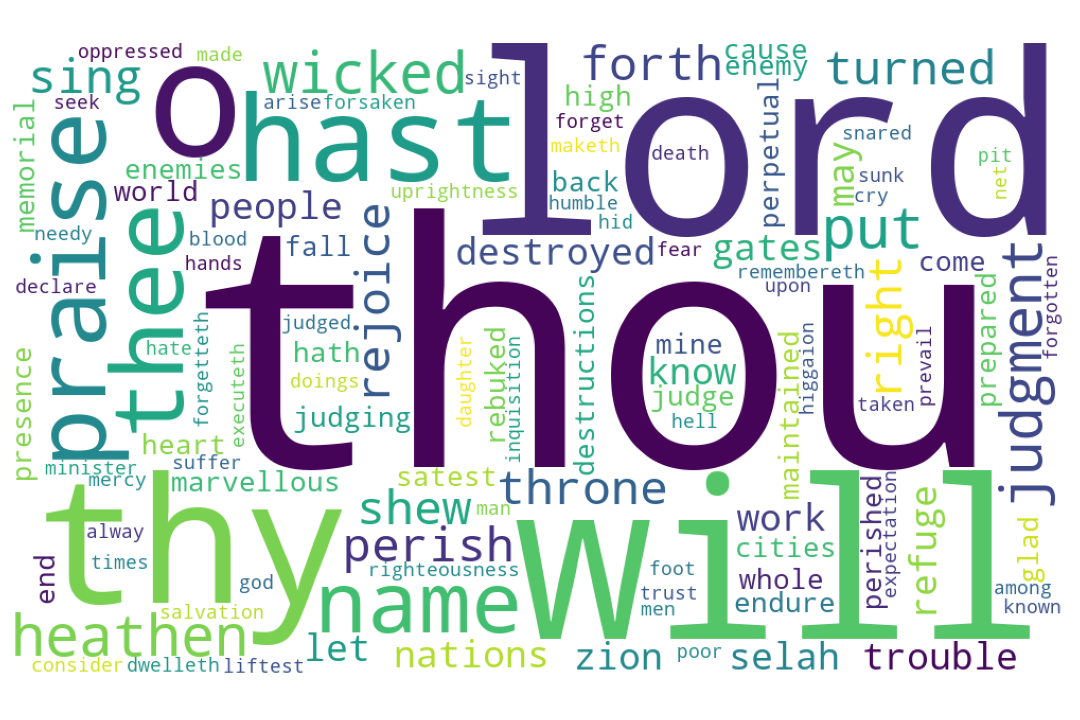
\includegraphics[width=\linewidth]{19OT-Psalms/Psalm9-WordCloud.jpg}
  \caption{Psalm 9 Word Cloud}
  \label{fig:Psalm 9 word Cloud}
\end{figure}

\marginpar{\scriptsize \centering \fcolorbox{bone}{lime}{\textbf{MANKIND AND HIS PLACE}}\\ (Psalm 9:1-20) \begin{compactenum}[I.][8]
    \item My \textbf{Rejoicing} \index[scripture]{Psalms!Psa 009:02}(Psa 9:2)
    \item God's \textbf{Rebuke} \index[scripture]{Psalms!Psa 009:05}(Psa 9:5)
    \item God's \textbf{Righteousness} \index[scripture]{Psalms!Psa 009:08}(Psa 9:8)
    \item God's \textbf{Remembrance} \index[scripture]{Psalms!Psa 009:12}(Psa 9:12)
    \item God's \textbf{Relief} \index[scripture]{Psalms!Psa 009:13}(Psa 9:13) (notably, a choice for man is available in verse 13.  Accept the mercy of God or perish in your own efforts to attain goodness)
    \item Human \textbf{Result} \index[scripture]{Psalms!Psa 009:15}(Psa 9:15) (mankind perishes in his own traps)
    \item Mankind's \textbf{Reality} \index[scripture]{Psalms!Psa 009:20}(Psa 9:20) (This is the Genesis 10 problem: man takes himself far too seriously. But he is just a human, made from  clay.)
    \item God's \textbf{Reminders} \index[scripture]{Psalms!Psa 009:20}(Psa 9:20) (It is God's mercy that reminds man of his place.)
\end{compactenum}}

\footnote{\textcolor[cmyk]{0.99998,1,0,0}{\hyperlink{TOC}{Return to end of Table of Contents.}}}\footnote{\href{https://audiobible.com/bible/bible.html}{\textcolor[cmyk]{0.99998,1,0,0}{Psalms Audio}}}\textcolor[cmyk]{0.99998,1,0,0}{To the chief Musician upon Muth-labben, A Psalm of David.}\\
\\
\textcolor[cmyk]{0.99998,1,0,0}{I will praise \emph{thee}, O LORD, with my whole heart; I will shew forth all thy marvellous works.}
[2] \textcolor[cmyk]{0.99998,1,0,0}{I will be glad and \fcolorbox{bone}{lime}{rejoice} in thee: I will sing praise to thy name, O thou most High.}
[3] \textcolor[cmyk]{0.99998,1,0,0}{When mine enemies are turned back, they shall fall and perish at thy presence.}
[4] \textcolor[cmyk]{0.99998,1,0,0}{For thou hast maintained my right and my cause; thou satest in the throne judging right.}
[5] \textcolor[cmyk]{0.99998,1,0,0}{Thou hast \fcolorbox{bone}{lime}{rebuked} the heathen, thou hast destroyed the wicked, thou hast put out their name for ever and ever.}
[6] \textcolor[cmyk]{0.99998,1,0,0}{O thou enemy, destructions are come to a perpetual end: and thou hast destroyed cities; their memorial is perished with them.}
[7] \textcolor[cmyk]{0.99998,1,0,0}{But the LORD shall endure for ever: he hath prepared his throne for judgment.}
[8] \textcolor[cmyk]{0.99998,1,0,0}{And he shall judge the world in \fcolorbox{bone}{lime}{righteousness}, he shall minister judgment to the people in uprightness.}
[9] \textcolor[cmyk]{0.99998,1,0,0}{The LORD also will be a refuge for the oppressed, a refuge in times of trouble.}
[10] \textcolor[cmyk]{0.99998,1,0,0}{And they that know thy name will put their trust in thee: for thou, LORD, hast not forsaken them that seek thee.}
[11] \textcolor[cmyk]{0.99998,1,0,0}{Sing praises to the LORD, which dwelleth in Zion: declare among the people his doings.}
[12] \textcolor[cmyk]{0.99998,1,0,0}{When he maketh inquisition for blood, he \fcolorbox{bone}{lime}{remembereth} them: he forgetteth not the cry of the humble.}
[13] \textcolor[cmyk]{0.99998,1,0,0}{Have mercy upon me, O LORD; consider my trouble \emph{which} \emph{I} \emph{suffer} of them that hate me, thou that liftest me up from the gates of death:}
[14] \textcolor[cmyk]{0.99998,1,0,0}{That I may shew forth all thy praise in the gates of the daughter of Zion: I will rejoice in thy salvation.}
[15] \textcolor[cmyk]{0.99998,1,0,0}{The heathen are sunk down in the pit \emph{that} they made: in \fcolorbox{bone}{lime}{the net which they hid} is their own foot taken.}
[16] \textcolor[cmyk]{0.99998,1,0,0}{The LORD is known \emph{by} the judgment \emph{which} he executeth: the wicked is snared in the work of his own hands. Higgaion. Selah.}
[17] \textcolor[cmyk]{0.99998,1,0,0}{The wicked shall be turned into hell, \emph{and} all the nations that forget God.}
[18] \textcolor[cmyk]{0.99998,1,0,0}{For the needy shall not alway be forgotten: the expectation of the poor shall \emph{not} perish for ever.}
[19] \textcolor[cmyk]{0.99998,1,0,0}{Arise, O LORD; \fcolorbox{bone}{lime}{let not man prevail}: let the heathen be judged in thy sight.}
[20] \textcolor[cmyk]{0.99998,1,0,0}{\fcolorbox{bone}{lime}{Put them in fear}, O LORD: \emph{that} the nations may know themselves \emph{to} \emph{be} \emph{but} men. Selah.}



